\appendix
\chapter{Appendix}
\label{sec:appendix}

\section{Initial guessing methods in \textsc{PySCF} \parencite{ref:pyscf}}
\label{sec:pyscf_initial_guessing_methods}
The \textsc{PySCF} package offers a variety of initial guessing methods for the density matrix for SCF calculations as described in the excerpt of the documentation \parencite{ref:pyscf_user_guide} bellow: 
\begin{itemize}
    \item \texttt{minao} (default): A superposition of atomic densities \parencite{ref:minao_sad1,ref:minao_sad2} technique, in which the guess is obtained by projecting the minimal basis of the first contracted functions in the cc-pVTZ or cc-pVTZ-PP basis set onto the orbital basis set, and then forming the density matrix. The guess orbitals are obtained by diagonalizing the Fock matrix that arises from the spin-restricted guess density.

    \item \texttt{1e}: The one-electron guess, also known as the core guess, obtains the guess orbitals from the diagonalisation of the core Hamiltonian, thereby ignoring all interelectronic interactions and the screening of nuclear charge. The 1e guess should only be used as a last resort, because it is so bad for molecular systems; see \parencite{ref:Lehtola2019}.

    \item \texttt{atom}: Superposition of atomic densities \parencite{ref:minao_sad1,ref:minao_sad2}. Employs spin-restricted atomic HF calculations that use spherically averaged fractional occupations with ground states determined by fully numerical calculations at the complete basis set limit in \parencite{ref:lethola_fully_numerical_atomic_potentials}.

    \item \texttt{huckel}: This is the parameter-free Hückel guess described in \parencite{ref:Lehtola2019}, which is based on on-the-fly atomic HF calculations performed analogously to \texttt{atom}. The spherically averaged atomic spin-restricted Hartree-Fock calculations yield a minimal basis of atomic orbitals and orbital energies, which are used to build a Hückel-type matrix that is diagonalized to obtain guess orbitals.

    \item \texttt{vsap}: Superposition of atomic potentials as described in \parencite{ref:Lehtola2019}. A sum of pre-tabulated, fully numerical atomic potentials determined with the approach of \parencite{ref:lethola_fully_numerical_atomic_potentials} is used to build a guess potential on a DFT quadrature grid; this potential is then used to obtain the orbitals. Note: this option is only available for DFT calculations in PySCF.
\end{itemize}



\section{Comments on second order Newton-solvers \& iterations}
\label{sec:notes_on_so_newton}
A second order Newton-solver essentially uses the Newton algorithm to converge an electron density by constructing density gradients $g$ and approximating the Hessian $H$ of the energy. The implementation in PySCF uses an outer macro loop which takes the newton steps and an inner loop which approximates the solution to the linearized Newton equation:
\[H \Delta x = -g\]
to obtain the update $\Delta x$ which is to be applied to the orbitals.\\

Faster convergence in terms of iterations was claimed by Schütt et al. for their neural network. \parencite{ref:schuett_unifying_2019} This prompted investigations on the \ch{C7H10O2} isomer set. Given our test set a comparable reduction of iterations from 1$^\text{st}$ order in \autoref{fig:dummy_iterations_qm9_isomers} to 2$^\text{nd}$ order\footnote{using PySCF's \texttt{newton\_ah} solver} in \autoref{fig:so_macro_iterations} can be seen. 

\begin{figure}[H]
    \centering
    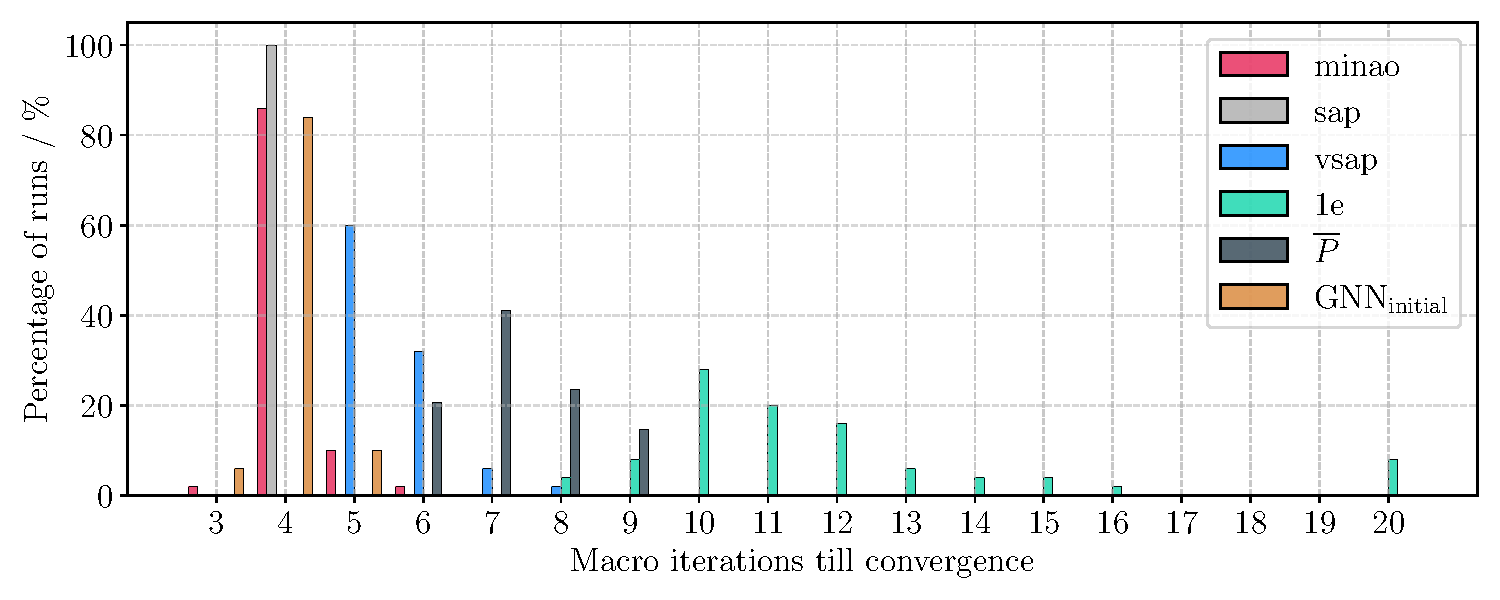
\includegraphics[width=\textwidth]{../fig/gnn/SO_0D_GNN_model_iteration_count_bar.pdf}
    \caption[Macro iterations till convergence distribution for QM9-isomers]{Macro iterations till convergence distribution for QM9-isomers for PySCF, $\overline{P}$ and GNN$_\text{initial}$ guesses. All entries with $\geq 20$ macro iterations are grouped at $20$.}
    \label{fig:so_macro_iterations}
\end{figure}
Yet this direct comparison is not a fair one. Contrary to DIIS, which builds the Fock matrix once per iteration, the Newton-solver repeatedly rebuilds the Fock matrix in it's inner loop. Summing all Fock matrix builds one obtains different behavior depicted in \autoref{fig:so_fock_build_iterations}.  
\begin{figure}[H]
    \centering
    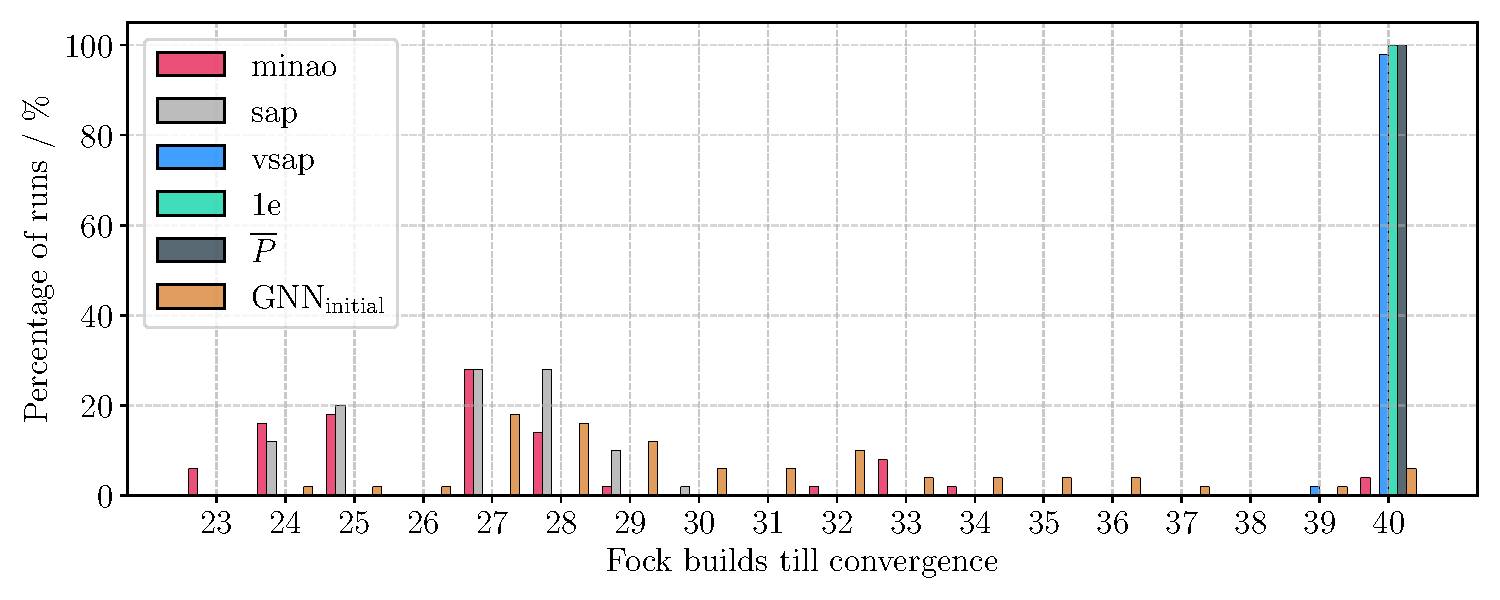
\includegraphics[width=\textwidth]{../fig/gnn/SO_0D_GNN_model_fock_build_count_bar.pdf}
    \caption[Fock matrix build count till convergence QM9-isomers]{Fock matrix build count till convergence for QM9-isomers for PySCF, $\overline{P}$ and GNN$_\text{initial}$ guesses. All entries with $\geq 40$ fock builds are grouped at $40$.}
    \label{fig:so_fock_build_iterations}
\end{figure}
Given this fact, one needs to be caution in making prediction regarding wall clock time of simulations from 'iteration` counts, especially for comparisons of different algorithms.

\section{Source Code \& Packages used}
\label{sec:source_code_packages}
\TODO{Remarks + references to code and packages used}